\chapter{Methode}
%
Zur Bearbeitung der Fragestellung wurde im Umfang dieser Arbeit ein firmeninternes Pilotprojekt durchgeführt, bei dem spiroergometrische Testmessungen mit unterschiedlichen internen und externen Probanden stattfanden. Im Vorwege wurden Einschluss- und Ausschlusskriterien sowie Bedingungen zur Vorbereitung erarbeitet, welche bei allen Testpersonen gleichermaßen eingehalten wurden. Eingeladen waren gesunde Menschen zwischen 18 und 60 Jahren, zu denen Sportler und Nicht-Sportler sowie Raucher und Nichtraucher zählten. Die Daten der Teilnehmer des Projektes sind unter Kapitel 2.5 aufgeführt. Mit den Messwerten wurden Grafiken generiert, anhand derer die ventilatorischen Schwellen zu bestimmen waren.
%
\section{Material \& Testaufbau}
%
Für die Tests wurde das \textsl{motion cycle 200med} der Firma \textsl{Emotion Fitness} genutzt, welches seriell mit einem Laptop und der \gls{CCPS} verbunden wird. Zur Abklärung der kardialen Gesundheit wurde der \textsl{cardioscan cs-3 effect} genutzt. Dies ist das firmeneigene MPG-zertifizierte Gerät zur Erstellung von \myglsgen{EKG} mittels vierer Klebe-Elektroden, mit dem die \gls{HF} in Ruhe und der \gls{CSI} erhoben werden. Für alle Tests wurde ein kalibriertes Modell des metabolicscan genutzt. Die Respirationsmessung erfolgt beim metaboliscan durch eine Atemeinheit, welches über ein Kabel und einen Probenschlauch mit der Analyseeinheit des Gerätes verbunden ist. Dieses sowie der Laptop und der cs-3 effect stehen darum auf einem Tisch in unmittelbarer Nähe zum Ergometer. Die Atemeinheit wird vor jeder Messung mit einem unbenutzten antibakteriellen Polypropylen-Filter des Herstellers \textsl{GVS} und einem dazugehörigen flexiblen Elastomer-Mundstück versehen. Jenes dient der Möglichkeit, das Atemmodul mit der Kiefermuskulatur festzuhalten, sodass die Hände während einer Messung am Ergometer bleiben können.
\clearpage
\subsection{Funktionsweise des metabolicscan}
%
Der metabolicscan besteht aus zwei Modulen: dem Atemmodul und der Analyseeinheit. Im Atemmodul des metabolicscan ist ein Flowsensor\footnote{Technische Daten: siehe Anhang A} verbaut. Dieser misst in direkter Nähe zum Mund die Strömungsgeschwindigkeit der Inspirations- bzw. Exspirationsluft in einem Bereich von $\pm$\SI{300}{S\litre\per\minute} mit einer Abtastrate von einer Millisekunde. Mithilfe einer mathematischen Integration über der Zeit wird anschließend das Strömungsvolumen berechnet. \gls{O2}- und \gls{CO2}-Sensor\footnote{Technische Daten: siehe Anhang B} sind in der separaten Analyseeinheit implementiert. Sie bilden ein optimal aufeinander abgestimmtes Modul und müssen daher für die Messung nicht zeitlich synchronisiert werden. Ein Anteil der Luft wird am Ende des Flowsensors über den Probenschlauch durch die integrierte Pumpe des \gls{CO2}-Sensors angesaugt. Die Funktion des \gls{CO2}-Sensors basiert auf Messung der Infrarotlichtabsorption durch \gls{CO2}, die im Spektralbereich von \SIrange{4,2}{4,3}{\micro\metre} besonders stark ist. Er eignet sich für eine \gls{AF} bis zu \SI{150}{\per\minute}, was ausreicht, da diese bei einer Spiroergometrie selten höher als \SI{60}{\per\minute} ansteigt~\cite{Hollmann.2006}. Anschließend wird die angesaugte Luft zum galvanischen \gls{O2}-Sensor geleitet. Dieser hat im Konzentrationsbereich von 0 bis 40 \% eine Genauigkeit von $\pm$~ (1~ \%\textsubscript{abs} + 1 \%\textsubscript{rel}), solange die \gls{AF} \SI{60}{\per\minute} nicht überschreitet.
%
\begin{figure}[H]
	\centering
	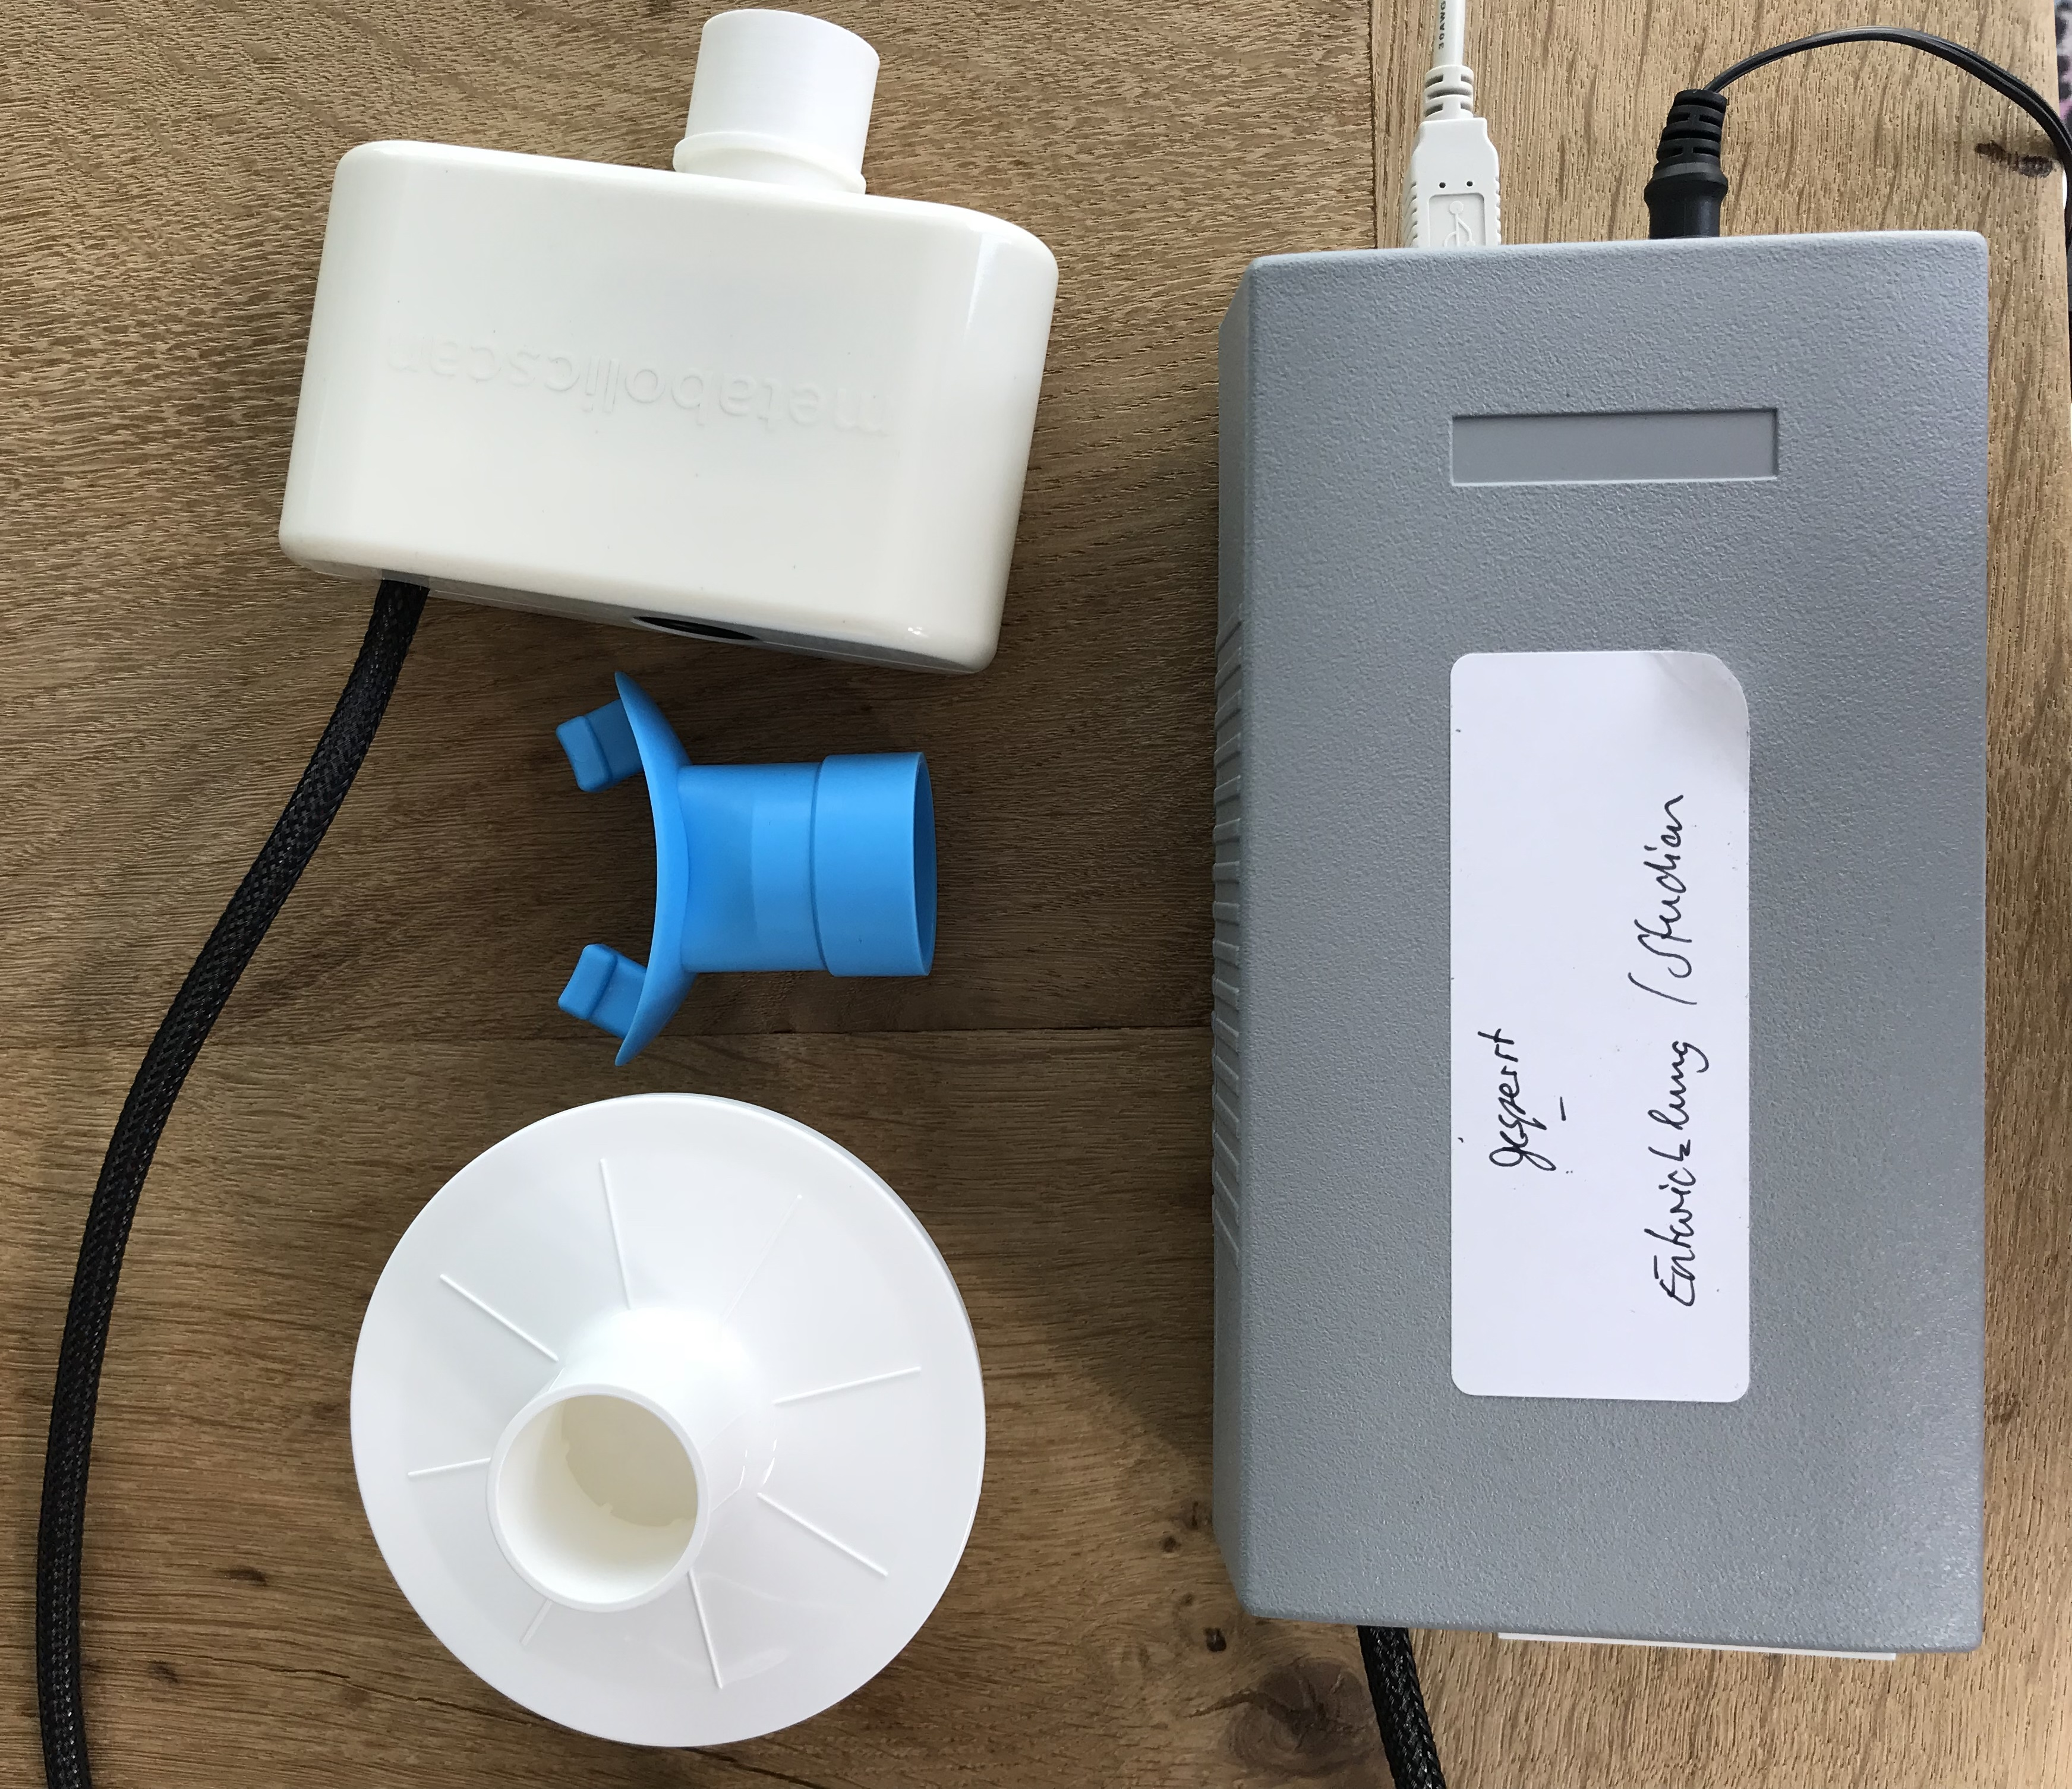
\includegraphics[width=100mm]{Bilder/mbs.jpg}
	\caption[metabolicscan: Analyseeinheit, Atemmodul, Filter und Mundstück]{metabolicscan: Analyseeinheit (rechts), Atemmodul (oben links), Filter (unten links) und Mundstück (blau)}
	\label{pic:pic9}
\end{figure}
%
\subsection{Messbedingungen}
%
Um gleichwertige Grundbedingungen zu schaffen, fanden alle Messungen in demselben Raum statt und es wurde darauf geachtet, dass die Raumtemperatur zwischen \SIlist{18;22}{\degreeCelsius} betrug, da diese sich auf die Herzfrequenz und Laktatakkumulation auswirken kann~\cite{Marino.2001}. Außerdem wurde der Raum vor jedem Test gut durchlüftet, um den \gls{CO2}-Anteil der Luft zu minimieren. Der metabolicscan wurde mindestens zehn Minuten vor dem ersten Test eingeschaltet, da sich die Sensoren kalibrieren und aufheizen müssen.
Als generelle Ausschlusskriterien für Probanden waren akute fiebrige Infekte, Herz-Kreislauf-Erkrankungen, chronische Atemwegserkrankungen (z.B. COPD) und Schwangerschaft festgelegt. Alle Teilnehmer erhielten bei Terminvergabe einen Informationsbogen, in dem sie unter anderem darüber aufgeklärt wurden, dass am Vortag auf anstrengende Sporteinheiten verzichtet werden sollte und ab zwei Stunden vor der Messung keine Mahlzeiten mehr eingenommen werden durften, da vor allem zuckerhaltige Lebensmittel kurz vor einer Messung neben dem RQ auch den Grund-Laktat-Spiegel erhöhen und somit das Messergebnis verfälschen~\cite{Ivy.1981}. Auch auf Koffein sollte in diesem Rahmen wegen eventueller Entzugserscheinungen verzichtet werden~\cite{Kroidl.2015}. Beim Fahrradergometer kann die Belastungsintensität neben der voreingestellten Leistung auch noch durch die Trittfrequenz beeinflusst werden. Damit die Intensität möglichst artefaktfrei gemäß des Belastungsprotokolls inkrementiert wird, sollte deshalb jeder Proband eine Trittfrequenz zwischen \SIlist{70;90}{\per\minute} beibehalten~\cite{Wonisch.2008}.
%
\section{Durchführung der Messungen}
%
\subsection{Vorbereitung \& Erwartungswerte}
%
Unmittelbar vor einem Test wurden die Probanden ein weiteres Mal über die Durchführung sowie eventuelle Risiken informiert und hatten eine Einwilligungserklärung zu unterzeichnen. Anschließend wurde ein Anamnesebericht ausgefüllt. Dafür wurden zunächst die Körpergröße sowie das Körpergewicht mithilfe der Ultraschallmessstation \textsl{seca 287} ermittelt. In Folge eines kurzen Interviews wurde der Trainings- und Gesundheitszustand der Person notiert. Mit dem cs-3 effect wurde ein zweiminütiges Ruhe-\gls{EKG} erstellt. Danach konnten durch die \gls{CCPS} Auffälligkeiten der \gls{HF} und des Herzrhythmus im Ruhezustand detektiert und betroffene Personen ggf. abgelehnt werden. Zur Erfassung der \gls{HF} während der Belastungsphase wurde ein Pulsgurt der Firma \textsl{Polar} angelegt, welcher mit dem Ergometer und der Software kommuniziert. Der Sattel des Ergometers war individuell für jeden Probanden ungefähr auf Hüfthöhe zu positionieren, sodass der Kniewinkel nicht mehr als $90$ \textdegree{} betrug, da dies eine höhere muskuläre Belastung beim Treten bewirken kann.
%
\subsubsection{Berechnung der maximalen Leistung}
%
Wie die Bezeichnung "`Leistungsdiagnostik"' bereits suggeriert, ist es enorm wichtig, dass die gemessene Person bis an ihr individuelles Leistungsmaximum gelangt, damit beide Schwellen vollwertig identifiziert werden können. Aus diesem Grund wurde vor einem Test ein individuelles Belastungsprotokoll für den Probanden erstellt. Den ersten Schritt stellte die Berechnung der \myglsgen{Wmax} in \si{\watt} dar, mit dem ein mindestens zu erwartender Wert bestimmt werden konnte. In der \gls{SHIP} sowie Studien nach Jones wurden Formeln für die Berechnung der Soll-Leistung erarbeitet. Nach SHIP~\cite{Koch.2009}:
%
\begin{flalign}
W_{max} (\male) &= -103,512 - 1,5766 * age + 2,2114 * \left\lbrace h\right\rbrace  \text{in \centi\metre} - 0,1198 * \left\lbrace m\right\rbrace \text{in \kilogram}
\label{eq:formel9}\\[1em]
W_{max} (\female) &= -80,628 - 0,7698 * age + 1,4038 * \left\lbrace h\right\rbrace \text{in \centi\metre} + 0,2873 * \left\lbrace m\right\rbrace \text{in \kilogram}
\label{eq:formel10}
\end{flalign}
%
Nach Jones (inklusive tolerierter Streuung von $\pm$18 \%)~\cite{Kroidl.2015}:
%
\begin{flalign}
W_{max} (\male) &= (2526 * \left\lbrace h\right\rbrace \text{in \metre} - 9,08 * age - 2759) * 0,163
\label{eq:formel11}\\[1em]
W_{max} (\female) &= (950 * \left\lbrace h\right\rbrace \text{in \metre} - 9,21 * age - 756) * 0,163
\label{eq:formel12}
\end{flalign}
%
Die folgenden Rechnungen zeigen die Anwendung bei einer weiblichen Probandin (w, 19) als Beispiel:
%
\begin{flalign*}
W_{max} &= -80,628 - 0,7698 * 19 + 1,4038 * 172\centi\metre - 0,2873 * 67\kilogram = 166\watt\\[1em]
W_{max} &= (950 * 1,72\metre - 9,21 * 19 - 756) * 0,163 = 181\watt \pm18\%
\end{flalign*}
%
Die Differenz zwischen den beiden Sollwerten ist mit \SI{15}{\watt} recht gering. Da beide Rechnungen offiziell empfohlen werden, wurde in dieser Arbeit dennoch bei allen Messungen mit beiden Formeln gerechnet und dann ein Mittelwert aus jedem Ergebnis gebildet~\cite{Kroidl.2015}. Für diese Probandin betrüge die maximale Belastungsintensität, welche abhängig von Alter und Körperdaten auch im untrainierten Zustand bewältigt werden kann, somit theoretisch \SI{174}{\watt}. Der Trainingszustand einer Person wurde bei der Bestimmung des Belastungsprotokolls berücksichtigt.
%
\subsubsection{Individuelles Belastungsprotokoll}
%
Mithilfe der maximalen Belastungsintensität wurde anschließend das Stufenprotokoll festgelegt. Die Dauer einer Belastungsstufe betrug zwei Minuten, wobei während der letzten \SI{30}{\second} einer Stufe die respiratorischen Werte erfasst wurden. Empfehlungen für Tests auf Fahrradergometern liegen zwischen \SIlist{7;26}{\minute} Gesamtdauer~\cite{Midgley.2008}. Darum wurde mit $n = 6$ ein Minimalwert für die zu bewältigenden Stufen \`{a} \SI{2}{\minute} bestimmt, da die Dauer eines Test somit \SI{12}{\minute} betrug und die Gefahr einer unzureichenden kardiorespiratorischen Ausbelastung reduziert wurde~\cite{Wonisch.2008}. Es war allerdings bei trainierten Personen davon auszugehen, dass sie die Soll-Belastung übertreffen und daher mehr als sechs Stufen ertragen. Deshalb wurde diese Zahl nur als ungefährer Richtwert verwendet. Als Inkrement wurde das Schema der \gls{WHO} mit \SI{25}{\watt} Steigerung je Stufe eingestellt. Dieser Standard galt für untrainierte wie trainierte Probanden, da hiermit eine Ausbelastung weitestgehend erreichbar sei~\cite{Trappe.2000}. Um die passende Anfangsbelastung zu bestimmen, wurde beispielsweise nach folgender Rechnung gearbeitet:
%
\begin{equation}
W_{Start} = W_{max} \text{(berechnet)} - 6 * 25 \watt 
\label{eq:formel13}
\end{equation}
%
Für die vorherige Beispielprobandin (w, 19) gilt dann:
%
\begin{equation*}
W_{Start} = 174\watt - 6 * 25\watt = 174\watt - 150\watt = 24\watt
\end{equation*}
%
Da diese Intensität allerdings nur minimal über der Leerlast durch den Eigenwiderstand des Ergometers mit \SI{15}{\watt} liegt, wurde bei dieser Probandin sowie bei allen weiteren sportlich aktiven Personen das Schema des \myglsgen{BAL} angewandt und eine Anfangsbelastung von \SI{50}{\watt} oder höher gewählt~\cite{Trappe.2000}. Dennoch wurde stets darauf geachtet, jene nicht zu überschätzen und damit eine muskuläre Erschöpfung vorzuziehen. Das Protokoll wurde schließlich in einen Softwaredialog der \gls{CCPS} eingepflegt. In dem Dialog war die Einstiegsbelastung gemäß der Berechnungen mit Berücksichtigung des Trainingszustands, das Inkrement mit \SI{25}{\watt}, die Stufendauer mit \SI{1,5}{\minute} sowie das Messintervall mit \SI{30}{\second} einzutragen. Generell ist bei keinem Menschen vorhersehbar, welche Anfangsbelastung und welches Inkrement optimal sind. Neben der körperlichen Leistungsfähigkeit spielt vor allem die persönliche Motivation bei der Durchführung des Tests eine wichtige Rolle~\cite{Kroidl.2015}. Daher mussten Abbruchkriterien definiert werden, die als Indiz für Ausbelastung gelten können.
%
\subsubsection{Abbruchkriterien}
%
Es wurden Abbruchkriterien nach Empfehlungen von Finger et al. festgelegt~\cite{Finger.2013}:
%
\begin{itemize}
	\item fallende Herzfrequenz trotz weiter steigender Belastung (>\SI{30}{\second})
	\item allgemeine Herzbeschwerden, Engegefühl in der Brust
	\item Atemnot
	\item auffällige Blässe
	\item akute Kopfschmerzen
	\item Schwindel oder Sehstörungen
	\item starke subjektive Erschöpfung
	\item Beinschwäche oder Muskelkrämpfe
	\item andauernder Abfall der Trittfrequenz unter \SI{60}{\per\minute}
\end{itemize}
%
Wurde die Intensität über die berechnete Soll-Belastung hinaus erhöht, galt dies nicht als Grund, den Test zu beenden~\cite{Wonisch.2008}. Indizien für eine kardiorespiratorische Ausbelastung waren eine einsetzende Plateauphase der \gls{VO2} oder der \gls{HF} trotz weiter ansteigender Belastung bzw. eine \gls{AF} >\SI{50}{\per\minute}~\cite{Kroidl.2015}. Diese Zustände dienten der objektiven Einschätzung des Zustandes eines Probanden. Vorwiegend wurde jedoch die eigene Beurteilung der Testperson berücksichtigt. 
%
\subsection{Leerlastphase}
%
Nach Vorbereitung einer Person wurde vor der Belastungsphase noch eine Referenzmessung des Stoffwechsels durchgeführt. Die Probanden hatten für ca. zwei Minuten in einer angenehmen Trittfrequenz gegen die Leerlast des Ergometers von \SI{15}{\watt} zu fahren. Dies ist eine gängige Methode, um venöse \gls{CO2}-Reste zu eliminieren und die verzögerte \gls{CO2}-Freisetzung aus dem Fettgewebe zu kompensieren. Damit wird der \gls{RQ} auf das möglichste Minimum reduziert~\cite{Kroidl.2015}. Nach Ablauf der zwei Minuten wurde eine Ruhestoffwechselmessung mit dem metabolicscan durchgeführt. Die momentane Programmierung der \gls{CCPS} setzt dies voraus, da mindestens acht Atemzüge als Referenz für die späteren Messungen bei Belastung notwendig sind. Anschließend konnte der Belastungstest gestartet und das voreingestellte Belastungsprotokoll durchfahren werden.
%
\subsection{Belastungsphase}
%
Während der Belastungsphase wurden die Probanden stetig unterstützt, indem ihnen die Atemeinheit gereicht und regelmäßig der momentane Zustand sowie die Belastungseinschätzung erfragt wurden. Außerdem wurde die Trittfrequenz überprüft und bei Bedarf daran erinnert, diese einzuhalten. Es wurde vor allem darauf geachtet, dass die Probanden rechtzeitig die Atemeinheit zur Hand hatten, um die Atemmessung durchzuführen. Die Software-Oberfläche der \gls{CCPS} zeigt während der Messung einen Timer an, welcher angibt, ab wann die nächste Messung gestartet wird. Zur korrekten Messwerterfassung war daher stets darauf zu achten, dass spätestens bei Ablauf des Timers das Mundstück vollständig im Mund war. Damit der gesamte Atem eines Probanden die Sensoren erreicht, muss zusätzlich vorher eine Nasenklammer aufgesetzt werden, um den ansonsten unkontrollierbar einsetzenden Teilvolumenstrom durch die Nase zu blockieren.
%
\begin{figure}[H]
	\centering
	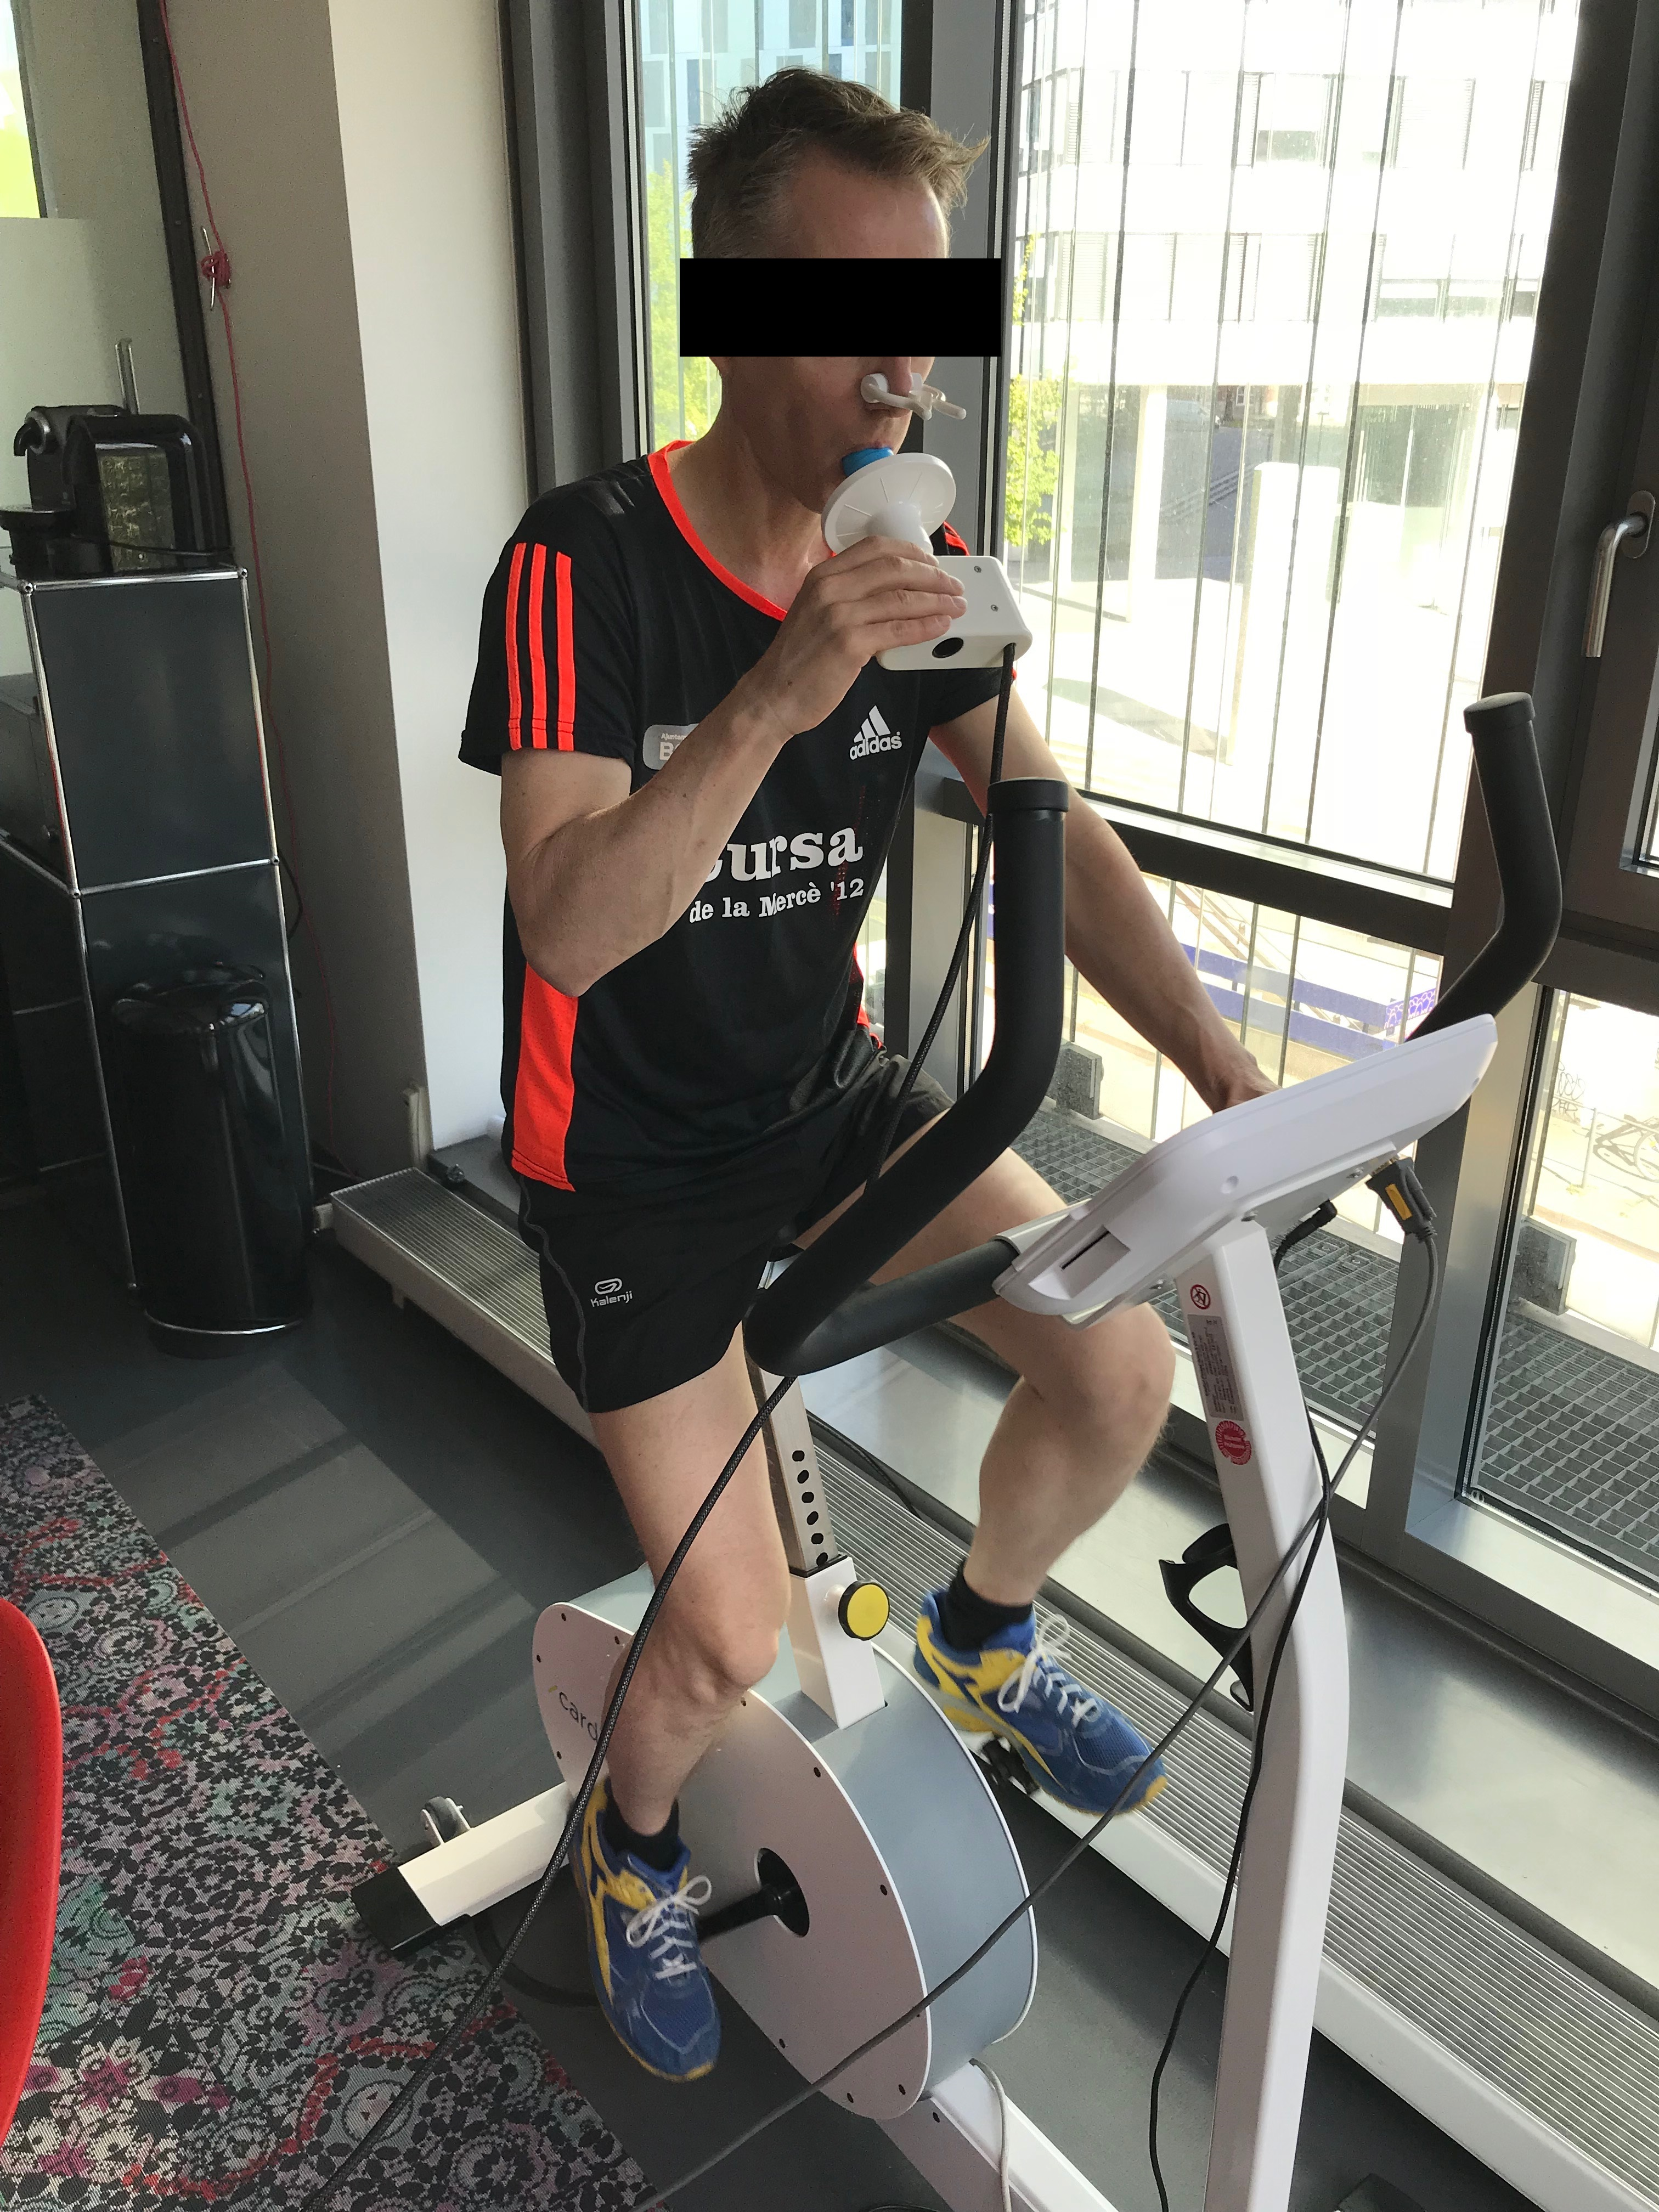
\includegraphics[width=90mm]{Bilder/proband.jpg}
	\caption{Proband während der Spiroergometrie}
	\label{pic:pic11}
\end{figure}
%
Abb. \ref{pic:pic11} zeigt beispielhaft einen männlichen Probanden während einer Spiroergometrie. Zu erkennen sind das verwendete Fahrradergometer, das Atemmodul, der Filter, das Mundstück und die Nasenklammer. Grundsätzlich war es den Probanden freigestellt, ob sie das Mundstück mit der Hand halten oder mit dem Kiefer. Eventuelle Auswirkungen des Handlings auf die Durchführung oder Ergebnisse werden in dieser Arbeit nicht behandelt.\\
In Abb. \ref{pic:pic12} ist die Oberfläche der \gls{CCPS} zu sehen, wie sie während einer Spiroergometrie auf dem Laptop dargestellt ist. Der Bildausschnitt zeigt die Graphen und Messwerte sowie den besagten Timer (oben in schwarzer Schrift) innerhalb eines Interfaces. Der obere rechte Plot zeigt die aktuell gemessene Durchflussrate des Flowsensors. Ist diese >0, handelt es sich um eine Exspiration, bei Werten <0 um eine Inspiration.
%
\begin{figure}[H]
	\centering
	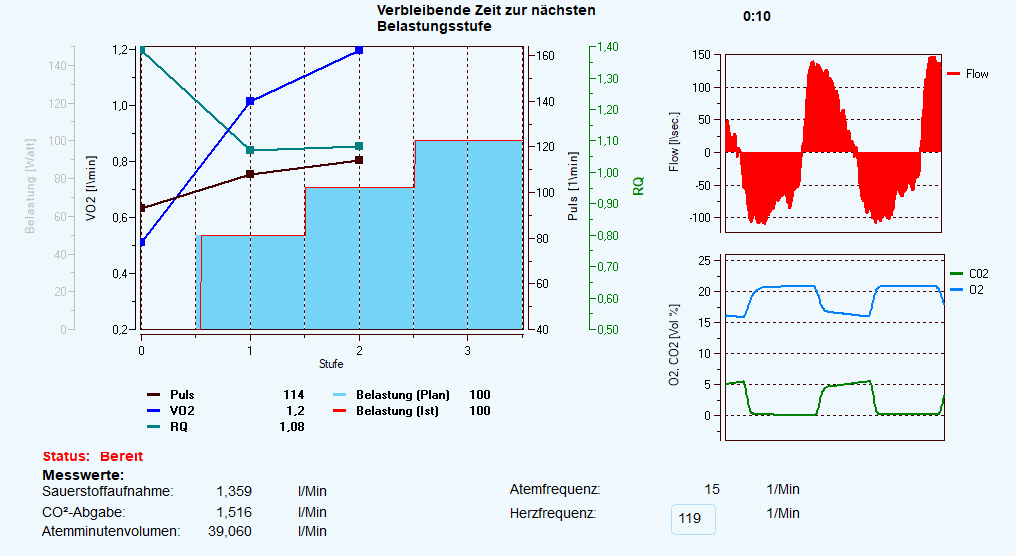
\includegraphics[width=\textwidth]{Bilder/sw_screen.png}
	\caption[Beispielhafte Software-Oberfläche während einer Spiroergometrie]{Beispielhafte Darstellung der \gls{CCPS}-Oberfläche während einer Spiroergometrie mit drei Plots. Links oben: Grafische Verlaufsdarstellung mehrerer Messwerte über die Belastungsstufen; Rechts oben: Darstellung des gemessenen Flows in \si{\litre\per\second}; Rechts unten: Prozentual gemessene \gls{O2}- (blau) und \gls{CO2}-Konzentration (grün)}
	\label{pic:pic12}
\end{figure}
%
Rechts unten ist mit drei Sekunden Latenz ein Plot mit den \gls{O2}- und \gls{CO2}-Konzentrationen eines Atemzugs eingebunden. Der blaue Graph stellt die \gls{O2}-, der grüne die \gls{CO2}-Konzentration dar. Das große Fenster links oben bildet eine Verlaufsdarstellung mit Mittelwerten bestimmter Parameter ab. Anhand der X-Achse des Koordinatensystems sind Stufennummerierungen zu erkennen. Auf der linken Y-Achse sind die Belastung in \si{\watt} und die \gls{VO2} in \si{\litre\per\minute} und auf der rechten der Puls bzw. die \gls{HF} in \si{\per\minute} und der \gls{RQ} definiert. Im Plot sind in verschiedenen Farben sind die pro Stufe ermittelten Mittelwerte für die \gls{VO2} (blau), den Puls (braun) und den \gls{RQ} (türkis) in Form eines Graphen sowie die während einer Stufe eingestellten Leistung als Balkendiagramm (hellblau). Unterhalb des Plots werden die Durchschnittswerte für besagte Parameter visualisiert, die bei der zuletzt abgeschlossenen Stufe durch die Software ausgewertet wurden. Außerdem werden im unteren Abschnitt des hellblauen Interfaces die während des letzten erkannten Atemzugs berechneten Werte für die \gls{VO2}, \gls{VCO2}, das \gls{AMV} und die \gls{AF} mitgeschrieben. Des Weiteren wird die vom Pulsgurt, via Ergometer an die Software übermittelte \gls{HF} angezeigt. Mithilfe dieses Interfaces konnte der Verlauf der Spiroergometrie überwacht und verfolgt werden. Der Timer half bei der korrekten Durchführung der Atemzugerfassung und die Graphen gaben Aufschluss darüber, ob diese korrekt funktionierte. Die Rohdaten der Sensoren wurden im Hintergrund aufgezeichnet, in \acrshort{CSV}-Dateien abgespeichert und konnten anschließend mit MATLAB ausgewertet werden.
%
\section{Datenverarbeitung \& Generierung der Plots}
%
Mithilfe mehrerer MATLAB-Skripte wurden die Sensor-Rohdaten automatisiert eingelesen und zur weiteren Verarbeitung vorbereitet. Anschließend wurden die einzelnen Atemzüge anhand des Flows detektiert, für jede Belastungsstufe gemittelt und in eine Ausgabematrix geschrieben. Anhand dieser wurden die Mittelwerte in mehreren Bezugssystemen grafisch aufgetragen. Am Ende der Ausführung der MATLAB-Skripte wurden die Graphen für V-Slope, \gls{EQO2}/\gls{EQCO2}, \gls{VE}/\gls{VCO2}, \gls{RQ}, \gls{VE}/\gls{W} und \gls{VO2}/\gls{W} in eine übersichtliche und vereinfachte 6-Felder-Grafik eingefügt und als Bild-Datei gespeichert. 
%
\section{Auswertung \& Referenzierung der Ergebnisse}
%
Schlussendlich wurden alle Plots zunächst subjektiv ausgewertet und die ventilatorischen Schwellen händisch bestimmt. Dabei wurden die Grafiken auf in Kapitel 1.2.2 genannte Indikatoren für die Schwellen analysiert. Auch in der klinischen Spiroergometrie wird zumeist nach dem Mehr-Augen-Prinzip ausgewertet, weshalb unabhängig eine zweite Person die Ergebnisse analysierte, deren Ansichten in dieser Arbeit als Referenz dienen. Da cardioscan die Schwellenbestimmung auch in Zukunft automatisiert durch die Software durchführen lassen möchte, wurde das MATLAB-Programm durch Algorithmen für die automatische Auswertung der Graphen erweitert und als dritte Ergebnisreihe hinzugefügt. Als Referenz für die Resultate dienten die Erkenntnisse der HUNT 3 Fitnessstudie von Loe et al. aus dem Jahre 2014~\cite{Loe.2014}. Im Zuge einer algorithmischen Schwellenbestimmung wurden die Ergebnisse durch die Software mit diesen Daten verglichen und auf Plausibilität überprüft. Die HUNT 3 Studie wurde zwar auf Laufbändern durchgeführt und beide Schwellen wurden ausschließlich mit der V-Slope-Methode bestimmt, jedoch bestand sie aus einer breit gefächerten Teilnehmergruppe mit 4631 Probanden. Daher bezeichnen Loe et al. ihre Erkenntnisse als größte europäische Referenzdaten-Sammlung für kardiorespiratorische Werte bei gesunden Männern und Frauen. Die Ergebnisse der zwei Rater sowie der Software wurden anschließend verglichen und auf Differenzen analysiert.
%
\section{Probandendaten}
%
Tab. \ref{tab:tabelle3} listet die Probanden-Daten Geschlecht, Gewicht in \si{\kilogram}, Körpergröße in \si{\centi\metre}, Alter in Lebensjahren, sportliche Aktivität in \si{\hour} pro Woche und die eigene Aussage, ob man Raucher ist oder nicht, auf. Unter den 28 Probanden waren zwölf Frauen und 16 Männer sowie fünf Raucher. Das Gesamtdurchschnittsalter betrug 33 Jahre. Das durchschnittliche Alter der Männer lag bei 35, das der Frauen bei 29 Jahren. Unter den Testpersonen befanden sich fünf Leistungssportler, von denen einer Olympionik ist. Im Mittel lag die wöchentliche sportliche Aktivität der Männer bei sieben, die der Frauen bei sechs Stunden. Anzumerken ist, dass es sich bei diesen Zahlen um subjektive Einschätzungen der Personen handelt und eventuell nicht die realen Gegebenheiten widerspiegeln. Dies liegt daran, dass "`sportliche Aktivität"' nicht eindeutig definiert ist und einige Probanden keine festen Trainingszeiten besitzen und daher unregelmäßig zum Sport gehen. Die Angaben wurden genutzt, um das Belastungsprotokoll, wie in Kapitel 2.2.1 beschrieben, anzupassen.
%
\begin{table}[H]
	\centering
	\caption{Probandendaten}
	\medskip
	\begin{tabulary}{\textwidth}{L C C C C C C}
		\toprule
		ID & Geschlecht & Gewicht in \si{\kilogram} & Größe in \si{\centi\metre} & Alter & Raucher & Akt. in \si{\hour\per Woche} \\
		\midrule
		\midrule
		1w & w & 65 & 171 & 40 & nein & 3,5 \\
		2w & w & 66 & 166 & 21 & ja & 2,5 \\
		3w & w & 70 & 163 & 31 & nein & 18 \\
		4m & m & 71 & 174 & 48 & nein & 5,5 \\
		5w & w & 56 & 167 & 25 & nein & 2 \\
		6w & w & 75 & 168 & 45 & ja & 6 \\
		7m & m & 86 & 178 & 37 & nein & 3 \\
		8m & m & 79 & 185 & 29 & nein & 13 \\
		9m & m & 94 & 178 & 44 & nein & 4 \\
		10w & w & 64 & 161 & 28 & nein & 11,5 \\
		11m & m & 75 & 176 & 26 & nein & 4 \\
		12m & m & 71 & 181 & 32 & nein & 6 \\
		13m & m & 93 & 171 & 29 & nein & 8 \\
		14m & m & 84 & 181 & 25 & nein & 35 \\
		15m & m & 97 & 187 & 28 & nein & 8 \\
		16w & w & 81 & 169 & 28 & ja & 1,5 \\
		17w & w & 49 & 155 & 20 & nein & 9 \\
		18w & w & 67 & 172 & 19 & nein & 8 \\
		19w & w & 50 & 156 & 47 & nein & 2 \\
		20m & m & 63 & 178 & 21 & ja & 2 \\
		21m & m & 105 & 184 & 21 & nein & 2 \\
		22m & m & 85 & 171 & 43 & ja & 0 \\
		23w & w & 64 & 174 & 40 & nein & 6 \\
		24m & m & 72 & 173 & 49 & nein & 5 \\
		25m & m & 68 & 174 & 58 & nein & 5 \\
		26m & m & 76 & 183 & 34 & nein & 7,5 \\
		27m & m & 101 & 192 & 34 & nein & 5 \\
		28w & w & 69 & 169 & 33 & nein & 3 \\
		\bottomrule
	\end{tabulary}
	\label{tab:tabelle3}
\end{table}